\subsection{Étude de la longueur de pétale selon les différentes espèces}
\subsubsection*{Représentations graphiques}
\vspace{.2cm}

%%%%%
\noindent
\textbf{Question~5~:} Représenter sur une même figure, les trois histogrammes de la longueur de pétale: un
histogramme pour chaque espèce avec une couleur. Commenter cette figure.
\vspace{.2cm}

\begin{figure}[!h]
    \centering
    \begin{minipage}{.48\linewidth}
        \begin{center}
            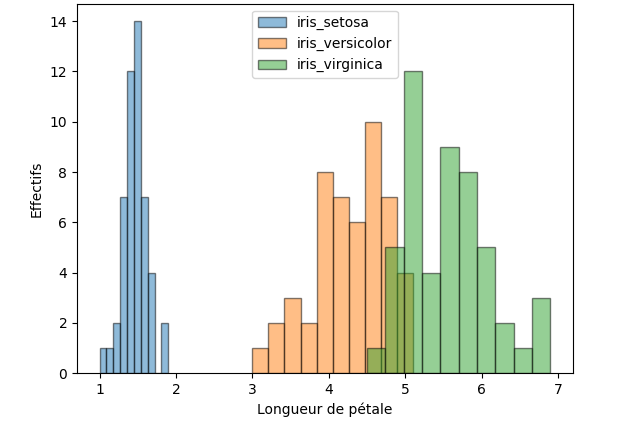
\includegraphics[width=1\textwidth]{img/Figure_3.png}
            \caption{\label{fig:figure3}Histogrammes de la longueur de pétale pour chaque espèce}
        \end{center}
    \end{minipage}\hfill
    \begin{minipage}{.48\linewidth}
        Lors du \textit{TP1 question 7}, nous avions pu remarquer que l'une des espèces a une taille de pétale plus faible, mais qui varie également moins que les deux autres. Le problème était que c'était seulement une hypothèse, puisque nous n'avions pas cette répartition 
        entre les différentes espèces. \\
        L'histogramme de la figure \ref*{fig:figure3}, reprend le même schéma que celui de la \textit{question~7 du TP1}, mais cette fois si en prenant en compte les différentes espèces. \\
        On peut donc conclure que notre hypothèse est vraie, l'iris setosa est plus petite que les deux autres espèces.
    \end{minipage}
\end{figure}

\begin{lstlisting}[style=myPython, caption=Code Python pour calculer le coefficient de corrélation, frame=lines]
iris_setosa_petallength = []
iris_versicolor_petallength = []
iris_virginica_petallength = []

for i in range(len(species)):
    if species[i] == 'Iris-setosa':
        iris_setosa_petallength.append(petallength[i])
    elif species[i] == 'Iris-versicolor':
        iris_versicolor_petallength.append(petallength[i])
    elif species[i] == 'Iris-virginica':
        iris_virginica_petallength.append(petallength[i])

plt.hist(iris_setosa_petallength, edgecolor='black', alpha=0.5, label='iris_setosa')
plt.hist(iris_versicolor_petallength, edgecolor='black', alpha=0.5, label='iris_versicolor')
plt.hist(iris_virginica_petallength, edgecolor='black', alpha=0.5, label='iris_virginica')
plt.xlabel('Longueur de pétale')
plt.ylabel('Effectifs')
plt.title("Histogrammes de la longueur de pétale pour chaque espèce")
plt.legend()
plt.show()
\end{lstlisting}

\vspace{.5cm}


%%%%%
\noindent
\textbf{Question~6~:} Représenter sur une même figure. une boite à moustache par espèce. Commenter cette
figure.
\vspace{.2cm}

\begin{figure}[!h]
    \centering
    \begin{minipage}{.66\linewidth}
        \begin{center}
            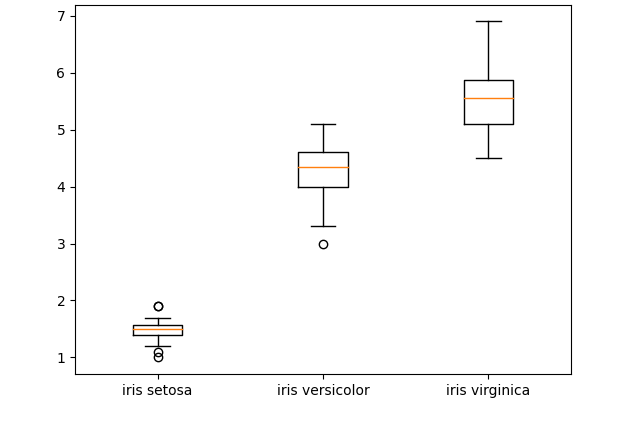
\includegraphics[width=1\textwidth]{img/Figure_4.png}
            \caption{\label{fig:figure4}Boite à moustache de la longueur de pétale pour chaque espèce}
        \end{center}
    \end{minipage}\hfill
    \begin{minipage}{.30\linewidth}
        On remarque encore une fois que l'iris setosa à un intervalle de longueur de pétales plus faible que les deux autres espèces.
    \end{minipage}
\end{figure}

\begin{lstlisting}[style=myPython, caption=Code Python pour calculer le coefficient de corrélation, frame=lines]
boxplot_petallength = [iris_setosa_petallength, iris_versicolor_petallength, iris_virginica_petallength]
plt.boxplot(boxplot_petallength, labels=['iris setosa', 'iris versicolor', 'iris virginica'])
plt.title("Boite à moustache de la longueur de pétale pour chaque espèce")
plt.show()
\end{lstlisting}

\clearpage

\subsubsection*{Représentations graphiques}
\vspace{.2cm}

%%%%%
\noindent
\textbf{Question~7~:} Calculer le rapport de corrélation lié à la décomposition de la variance en variance intraclasse et interclasse. Qu’en concluez-vous?
\vspace{.2cm}

\begin{enumerate}
    \item \textbf{Formules utilisées~:}
        \begin{figure}[!h]
            \centering
            \begin{minipage}{.49\linewidth}
                \begin{itemize}
                    \item[--] Variance interclasse~: 
                        \begin{equation}
                            S^2_{B} = \frac{1}{n} \sum_{i=1}^{p} n_{i}(\overline{Y_{i}} - \overline{Y})^2
                        \end{equation}
                \end{itemize}
            \end{minipage}\hfill\vline
            \begin{minipage}{.49\linewidth}
                \begin{itemize}
                    \item[--] Variance intraclasse~:
                        \begin{equation}
                            S^2_{W} = \frac{1}{n} \sum_{i=1}^{p} n_{i}.S^2_{n-1,Y_{i}}
                        \end{equation}
                \end{itemize}
            \end{minipage}
        \end{figure}

        \begin{itemize}
            \item[--] Variance totale~:
                \begin{equation}\label{eq:var_total}
                    S^2_{n-1,Y} = S^2_{B} + S^2_{W}
                \end{equation}
            \item[--] Rapport de corrélation~:
                \begin{equation}
                    S_{\frac{Y}{X}} = \sqrt{\frac{S^2_{B}}{S^2_{n-1,Y}}} \in [0 , 1]
                \end{equation}
        \end{itemize}

    \item \textbf{Valeurs obtenues~:}
    
        \vspace{.2cm}

        \begin{center}
            \begin{tabular}{| c | c |}
                \hline
                \textbf{Variance interclasse} & 2.910\\\hline
                \textbf{Variance intraclasse} & 0.181\\ \hline
                \textbf{Variance total} & 3.092\\ \hline
                \textbf{Rapport de corrélation} & 0.970\\ \hline


            \end{tabular}
        \end{center}

        \vspace{.5cm}

    \item \textbf{Conclusion~:}
    
        \vspace{.2cm}
        
        La variance totale trouvée grâce à la formule \ref*{eq:var_total}, correspond avec celle trouvée avec \textit{numpy}. Cette constatation nous permet de nous assurer que nos résultats sont corrects et de trouver par la suite le rapport 
        de corrélation qui est de 0,970. \\
        Le rapport de corrélation étant proche de 1 nous permet de confirmer notre hypothèse établie à la \textit{question~4} concernant la corrélation des variables \textit{petalLength} et \textit{petalWidth}.

        \vspace{.5cm}

    \item \textbf{Code python~:}
    
    \vspace{.2cm}

        \begin{lstlisting}[style=myPython, caption=Code Python pour calculer le coefficient de corrélation, frame=lines]
n_cumul = len(species)

mean_species_petallength = [np.mean(iris_setosa_petallength), np.mean(iris_versicolor_petallength), np.mean(iris_virginica_petallength)]

mean_petallength = np.mean(petallength)

var_species_petallength = [np.var(iris_setosa_petallength), np.var(iris_versicolor_petallength), np.var(iris_virginica_petallength)]

n_species = [len(iris_setosa_petallength), len(iris_versicolor_petallength), len(iris_virginica_petallength)]



def var_inter_classe_petallength(n_cumul, n_species, mean_species, mean):
    ret = 0
    for i in range(len(speciesname)):
        ret += n_species[i] * (mean_species[i] - mean)**2

    return ret/n_cumul



def var_intra_classe_petallength(n_cumul, n_species, var_species):
    ret = 0
    for i in range(len(speciesname)):
        ret += n_species[i] * var_species[i]

    return ret / n_cumul



var_inter_classe = var_inter_classe_petallength(n_cumul, n_species, mean_species_petallength, mean_petallength)

var_intra_classe = var_intra_classe_petallength(n_cumul, n_species, var_species_petallength)

var_totale_formule = var_inter_classe + var_intra_classe

var_totale = np.var(petallength)

rapport_corr = np.sqrt(var_inter_classe/var_totale_formule)

print("Variance interclasse: ", var_inter_classe)
print("Variance intraclasse: ", var_intra_classe)
print("Variance total trouvé avec la formule: ", var_totale_formule)
print("Variance total trouvé avec numpy: ", var_totale)
print("Rapport de corrélation: ", rapport_corr)
            \end{lstlisting}
            
            \begin{lstlisting}[style=myLog, caption=Résultat du code, frame=lines]
Variance interclasse:  2.910958222222223
Variance intraclasse:  0.1814666666666667
Variance total trouvé avec la formule:  3.0924248888888894
Variance total trouvé avec numpy:  3.092424888888889
Rapport de corrélation:  0.9702159417163924                
            \end{lstlisting}


\end{enumerate}




\clearpage